\documentclass{article}
\usepackage{fullpage}
\usepackage{graphicx}

\title{16.35 PSet \#2}
\author{Ryan Fish}
\date{\today}

\begin{document}
\maketitle

\section{Predeliverables}
\subsection{Test Case Rationale}

My addVehicle method simply adds a reference to the vehicle to a list of all vehicles so that it's state can be gathered later by the Simulator.  The important stuff happens upon construction of the vehicle and controller, where it adds itself to the set of threads that must run in lockstep with the time incrementation.  Since the predeliverable implementation is just wait for time, set speeds and update positions, I just check to make sure that adding a vehicle or controller increments the count, that getting the time decrements the count, and incrementing the time resets the count.

\subsection{No Noise, 5 Vehicles}

\begin{center}
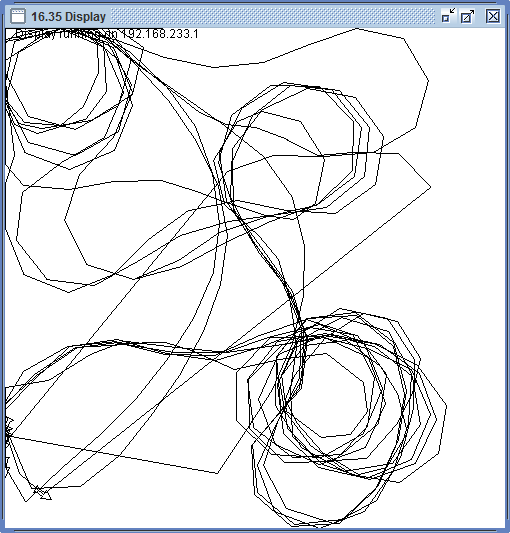
\includegraphics[width=0.7\linewidth]{5nonoise}
\end{center}

\subsection{Noise, 5 Vehicles}

\begin{center}
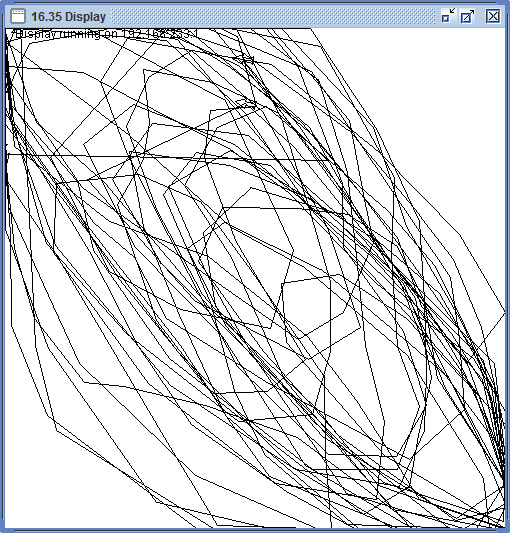
\includegraphics[width=0.7\linewidth]{5noise}
\end{center}


\subsection{4 Conditions of Deadlock and You}

\begin{enumerate}
	\item[MutEx] We need to prevent reads occurring concurrently with writes to vehicle state.
	\item[Hold and Wait] In particular, LeadingController may grab its own state and wait for a lock on the state of a vehicle it is leading.
	\item[No Preemption]  Without modification, the default synchronization system of Java does not allow for preemption in acquisition of resources.
	\item[Circular Wait]  A Leading Controller may wait on acquisition of the state of a Following controller, who is waiting to acquire the state of the same LeadingController.
\end{enumerate}
\subsection{Proposal for Avoiding Deadlock} 

The best way to attack deadlock in this scenario would be to attack circular wait.  I will build an object to manage monitor acquisition that will assign a monotonically increasing index to object classes able to be locked, and prevent acquisition of an index lower than the highest one held.  It will trigger a release of any objects held with higher indexes.

\end{document}
